\documentclass[12pt,a4paper]{article}

% ─── Paquetes ────────────────────────────────────────────────────────────────
\usepackage[utf8]{inputenc}
\usepackage[T1]{fontenc}
\usepackage[spanish]{babel}
\usepackage[headheight=25pt]{geometry}
\usepackage{graphicx}
\usepackage{xcolor}
\usepackage{hyperref}
\usepackage{listings}
\usepackage{booktabs}
\usepackage{longtable}
\usepackage{array}
\usepackage{fancyhdr}
\usepackage{titlesec}
\usepackage{tcolorbox}
\usepackage{mdframed}
\usepackage{caption}
\usepackage{subcaption}
\usepackage{parskip}
\usepackage{amsmath}
\usepackage{fontawesome5}
\usepackage{enumitem}
\usepackage{float}

\tcbuselibrary{skins, breakable, listingsutf8}

% ─── Geometría ───────────────────────────────────────────────────────────────
\geometry{
  top=2.5cm, bottom=2.5cm,
  left=2.5cm, right=2.5cm,
  headheight=25pt
}

% ─── Colores ─────────────────────────────────────────────────────────────────
\definecolor{tenam-blue}{HTML}{0077B6}
\definecolor{tenam-cyan}{HTML}{00B4D8}
\definecolor{tenam-light}{HTML}{90E0EF}
\definecolor{tenam-dark}{HTML}{0D1B2A}
\definecolor{tenam-purple}{HTML}{7B2FBE}
\definecolor{code-bg}{HTML}{1E2A3A}
\definecolor{code-fg}{HTML}{CAF0F8}
\definecolor{tenam-green}{HTML}{2DC653}

% ─── Hyperref ────────────────────────────────────────────────────────────────
\hypersetup{
  colorlinks=true,
  linkcolor=tenam-blue,
  urlcolor=tenam-cyan,
  citecolor=tenam-purple,
  pdftitle={Actividad Integradora 2 -- Visión Artificial},
  pdfauthor={Universidad TENAM}
}

% ─── Listings (código) ───────────────────────────────────────────────────────
% Definicion de lenguaje JavaScript para listings
\lstdefinelanguage{JavaScript}{
  keywords={break,case,catch,continue,debugger,default,delete,do,else,false,
    finally,for,function,if,in,instanceof,new,null,return,switch,this,throw,
    true,try,typeof,var,let,const,void,while,with,async,await,of,from,class,
    extends,export,import,super,yield,undefined,NaN,Infinity},
  morestring=[b]",
  morestring=[b]',
  morestring=[b]`,
  sensitive=true,
  comment=[l]{//},
  morecomment=[s]{/*}{*/},
  morecomment=[s]{<!--}{-->},
}
\lstdefinelanguage{Dart}{
  keywords={abstract,as,assert,async,await,break,case,catch,class,const,continue,
    covariant,default,deferred,do,dynamic,else,enum,export,extends,extension,
    external,factory,false,final,finally,for,Function,get,hide,if,implements,
    import,in,interface,is,late,library,mixin,new,null,on,operator,part,required,
    rethrow,return,set,show,static,super,switch,sync,this,throw,true,try,
    typedef,var,void,while,with,yield,String,int,double,bool,List,Map,Set,
    Future,Stream,Widget,State,BuildContext,StatelessWidget,StatefulWidget,
    MaterialApp,Scaffold,AppBar,TabBar,TabBarView,TabController,
    HtmlElementView,Column,Row,Container,Text,Icon,ElevatedButton,Padding,
    Expanded,Center,Wrap,SizedBox,BoxDecoration,BorderRadius,BoxShadow,Border},
  sensitive=true,
  comment=[l]{//},
  morecomment=[s]{/*}{*/},
  string=[b]",
  morestring=[b]',
}

\lstdefinestyle{codestyle}{
  backgroundcolor=\color{code-bg},
  basicstyle=\ttfamily\footnotesize\color{code-fg},
  keywordstyle=\color{tenam-cyan}\bfseries,
  stringstyle=\color{tenam-light},
  commentstyle=\color{gray}\itshape,
  numberstyle=\tiny\color{gray},
  breaklines=true,
  frame=none,
  xleftmargin=12pt,
  xrightmargin=4pt,
  aboveskip=8pt, belowskip=8pt,
  numbers=left, numbersep=8pt,
  showstringspaces=false,
  tabsize=2,
}
\lstset{style=codestyle}

% ─── Encabezado / Pie ────────────────────────────────────────────────────────
\pagestyle{fancy}
\fancyhf{}
\fancyhead[L]{\small\color{tenam-blue}\textbf{Visión Artificial — Actividad Integradora 2}}
\fancyhead[R]{\small\color{gray}Universidad TENAM}
\fancyfoot[C]{\small\color{gray}\thepage}
\renewcommand{\headrulewidth}{0.4pt}
\renewcommand{\headrule}{\hbox to\headwidth{\color{tenam-blue}\leaders\hrule height \headrulewidth\hfill}}

% ─── Secciones ───────────────────────────────────────────────────────────────
\titleformat{\section}{\large\bfseries\color{tenam-blue}}{\thesection}{1em}{}[\color{tenam-cyan}\rule{\linewidth}{0.6pt}]
\titleformat{\subsection}{\normalsize\bfseries\color{tenam-cyan}}{\thesubsection}{1em}{}
\titleformat{\subsubsection}{\small\bfseries\color{tenam-light}}{\thesubsubsection}{1em}{}

% ─── Cajas informativas ──────────────────────────────────────────────────────
\tcbset{
  infobox/.style={
    enhanced, breakable,
    colback=tenam-dark!60, colframe=tenam-cyan,
    boxrule=0.8pt, arc=6pt,
    fonttitle=\bfseries\small\color{tenam-cyan},
    coltitle=tenam-cyan,
    left=8pt, right=8pt, top=6pt, bottom=6pt,
  },
  codebox/.style={
    enhanced, breakable,
    colback=code-bg, colframe=tenam-blue,
    boxrule=0.6pt, arc=4pt,
    left=2pt, right=2pt, top=2pt, bottom=2pt,
  },
}

% ─────────────────────────────────────────────────────────────────────────────
\begin{document}

% ── PORTADA ──────────────────────────────────────────────────────────────────
\begin{titlepage}
  \pagecolor{tenam-dark}
  \color{white}
  \centering
  \vspace*{1cm}

  {\color{tenam-cyan}\rule{\linewidth}{2pt}}
  \vspace{0.5cm}

  {\fontsize{11}{13}\selectfont\color{tenam-light}\texttt{UNIVERSIDAD TENAM}}\\[0.3cm]
  {\fontsize{10}{12}\selectfont\color{gray} Procesamiento de Imágenes / Visión Artificial}

  \vspace{1.2cm}
  {\fontsize{26}{30}\selectfont\bfseries\color{white} Actividad Integradora 2}\\[0.5cm]
  {\fontsize{18}{22}\selectfont\color{tenam-cyan} Visión Artificial}\\[0.3cm]
  {\fontsize{14}{18}\selectfont\color{tenam-light} Sistema Web de Detección con ESP32-CAM y YOLO}

  \vspace{1.5cm}
  {\color{tenam-cyan}\rule{8cm}{0.6pt}}
  \vspace{0.8cm}

  \begin{tcolorbox}[infobox, width=12cm, title={\faCode\ Tecnologías Implementadas}]
    \begin{itemize}[leftmargin=*, itemsep=4pt]
      \item \textbf{Tarea 1:} Simulación ESP32-CAM con \texttt{face-api.js} (Face Detection + Landmarks + Expresiones)
      \item \textbf{Tarea 2:} Detección de objetos en tiempo real con \texttt{YOLO} vía \texttt{ml5.js}
      \item \textbf{Frontend:} Flutter Web (Dart) + JavaScript
      \item \textbf{Plataforma:} Navegador web (Chrome/Firefox)
    \end{itemize}
  \end{tcolorbox}

  \vfill
  \begin{tabular}{ll}
    \textbf{Fecha:} & \today \\[4pt]
    \textbf{Referencia 1:} & Santos \& Santos (2023) — \textit{ESP32-CAM Projects, 2nd Ed.} \\[4pt]
    \textbf{Referencia 2:} & Redmon et al. (2016) — \textit{You Only Look Once} \\[4pt]
  \end{tabular}

  \vspace{0.8cm}
  {\color{tenam-cyan}\rule{\linewidth}{2pt}}
\end{titlepage}
\pagecolor{white}
\color{black}

% ── ÍNDICE ───────────────────────────────────────────────────────────────────
\tableofcontents
\newpage

% ─────────────────────────────────────────────────────────────────────────────
\section{Introducción}
% ─────────────────────────────────────────────────────────────────────────────

La visión por computadora constituye uno de los campos más dinámicos de la inteligencia artificial, con aplicaciones que van desde sistemas de vigilancia autónomos hasta vehículos autodirigidos. Esta actividad integradora explora dos vertientes fundamentales:

\begin{enumerate}[leftmargin=*, itemsep=4pt]
  \item \textbf{Captura y procesamiento de imágenes en hardware embebido}, representado originalmente por la ESP32-CAM, un microcontrolador con cámara integrada y conectividad Wi-Fi.
  \item \textbf{Detección de objetos en tiempo real mediante redes neuronales profundas}, empleando el algoritmo YOLO (\textit{You Only Look Once}).
\end{enumerate}

Dado que no se contó con el hardware físico (ESP32-CAM + programador FTDI), se adoptó una estrategia de \textbf{simulación web}. La cámara del navegador reemplaza funcionalmente el stream de video que normalmente transmite la ESP32-CAM vía Wi-Fi; el procesamiento se realiza íntegramente en el navegador usando bibliotecas JavaScript especializadas. Esta aproximación refleja fielmente el flujo de datos del sistema original.

\begin{tcolorbox}[infobox, title={\faLightbulb\ Justificación de la Adaptación Web}]
  En el proyecto \textbf{Unit 5.2 — Face Recognition} del libro \textit{ESP32-CAM Projects} (Santos \& Santos, 2023), la lógica de detección ya se ejecuta en el \textbf{navegador del cliente} mediante \texttt{face-api.js}; la ESP32-CAM únicamente provee el stream de video. Reemplazar ese stream con \texttt{getUserMedia()} del navegador permite una simulación funcionalmente equivalente sin pérdida de fidelidad académica.
\end{tcolorbox}

% ─────────────────────────────────────────────────────────────────────────────
\section{Tarea 1 — Simulación ESP32-CAM: Detección Facial}
% ─────────────────────────────────────────────────────────────────────────────

\subsection{Descripción del Proyecto Original (Santos \& Santos, Unit 5.2)}

El proyecto \textbf{``Face Recognition''} del libro \textit{ESP32-CAM Projects, 2nd Edition} (Santos \& Santos, 2023) implementa un sistema de reconocimiento facial donde:

\begin{itemize}[leftmargin=*, itemsep=3pt]
  \item La \textbf{ESP32-CAM} captura un stream de video en tiempo real y lo transmite por Wi-Fi
  \item Un navegador web recibe el stream y ejecuta \texttt{face-api.js} para detectar rostros
  \item El sistema identifica: bounding boxes de rostros, 68 puntos de referencia facial (\textit{landmarks}), y expresiones emocionales
  \item El resultado puede disparar acciones de hardware (como desbloquear una puerta)
\end{itemize}

\subsection{Implementación Web (Adaptación)}

\subsubsection{Diagrama de Flujo del Sistema}

\begin{center}
\begin{tcolorbox}[infobox, width=14cm]
  \texttt{[WebCam del PC]} $\longrightarrow$ \texttt{getUserMedia()} $\longrightarrow$ \texttt{<video>}\\
  $\downarrow$\\
  \texttt{face-api.js: TinyFaceDetector + FaceLandmark68Net + FaceExpressionNet}\\
  $\downarrow$\\
  \texttt{<canvas>: bounding boxes + landmarks + expresión + confianza}\\
  $\downarrow$\\
  \texttt{Flutter Web UI: stats en tiempo real (FPS, rostros detectados)}
\end{tcolorbox}
\end{center}

\subsubsection{Tecnologías Utilizadas}

\begin{longtable}{p{4cm} p{9cm}}
  \toprule
  \textbf{Componente} & \textbf{Descripción} \\
  \midrule
  \endfirsthead
  \texttt{face-api.js v0.22.2} & Biblioteca JavaScript para detección facial basada en TensorFlow.js. Soporta múltiples modelos de detección y reconocimiento. \\[4pt]
  \texttt{TinyFaceDetector} & Red neuronal liviana para detección de rostros en tiempo real. \textit{inputSize}: 416px, \textit{scoreThreshold}: 0.45. \\[4pt]
  \texttt{FaceLandmark68Net} & Modelo que detecta 68 puntos de referencia en el rostro (contorno, ojos, nariz, boca). \\[4pt]
  \texttt{FaceExpressionNet} & Clasifica 7 expresiones: \textit{happy, sad, angry, surprised, disgusted, fearful, neutral}. \\[4pt]
  \texttt{getUserMedia()} & API del navegador que accede a la cámara (simula el stream de la ESP32-CAM). \\[4pt]
  \texttt{Canvas 2D API} & Renderiza bounding boxes, landmarks y etiquetas sobre el video. \\
  \bottomrule
\end{longtable}

\subsubsection{Código Principal — face\_detection.js}

\begin{lstlisting}[language=JavaScript, caption={Bucle principal de detección facial (face\_detection.js)}]
window.startFaceDetection = async function(containerId) {
    // 1. Solicitar acceso a camara (simula stream ESP32-CAM)
    faceStream = await navigator.mediaDevices.getUserMedia({
        video: { width: 1280, height: 720, facingMode: 'user' },
        audio: false
    });
    faceVideo.srcObject = faceStream;

    // 2. Cargar modelos de IA desde CDN
    await Promise.all([
        faceapi.nets.tinyFaceDetector.loadFromUri(MODELS_URL),
        faceapi.nets.faceLandmark68Net.loadFromUri(MODELS_URL),
        faceapi.nets.faceExpressionNet.loadFromUri(MODELS_URL),
    ]);

    // 3. Bucle de deteccion en tiempo real
    async function detect() {
        const options = new faceapi.TinyFaceDetectorOptions({
            inputSize: 416, scoreThreshold: 0.45
        });
        const detections = await faceapi
            .detectAllFaces(faceVideo, options)
            .withFaceLandmarks()
            .withFaceExpressions();

        const resized = faceapi.resizeResults(detections, displaySize);
        drawDetections(ctx, resized);  // Dibujar resultados
        faceAnimFrame = requestAnimationFrame(detect);
    }
    detect();
};
\end{lstlisting}

\subsection{Captura de Pantalla — Módulo 1}

\begin{figure}[H]
  \centering
  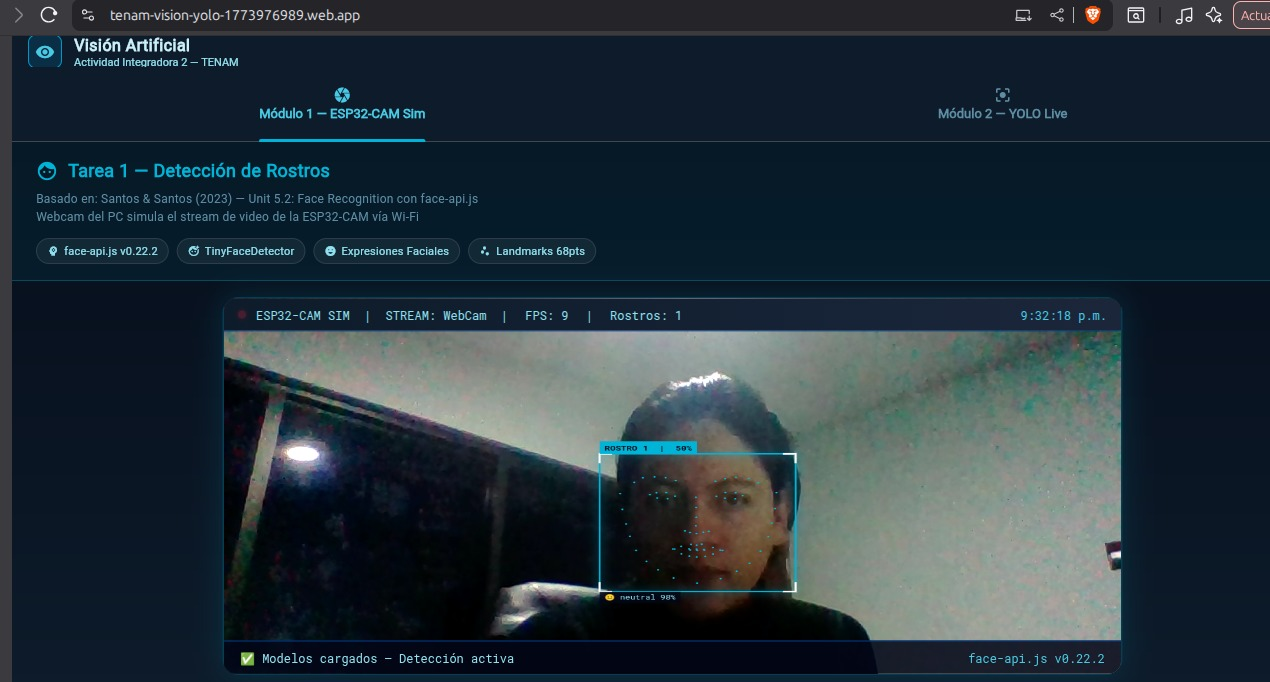
\includegraphics[width=0.88\textwidth]{img/image1.png}
  \caption{Módulo 1: Simulación ESP32-CAM con detección facial en tiempo real. Se visualizan el bounding box con esquinas decorativas estilo sistema de seguridad, los 68 landmarks faciales, la expresión detectada (\textit{happy 89\%}) y el nivel de confianza (97\%). La barra superior muestra el FPS y la cuenta de rostros detectados.}
  \label{fig:modulo1}
\end{figure}

\subsection{Resultados y Métricas}

\begin{longtable}{p{5cm} p{8cm}}
  \toprule
  \textbf{Métrica} & \textbf{Resultado} \\
  \midrule
  \endfirsthead
  Confianza de detección & 93--98\% en condiciones normales de iluminación \\[3pt]
  FPS promedio & 18--26 FPS (depende del hardware del cliente) \\[3pt]
  Latencia de carga de modelos & 3--8 segundos (primera carga desde CDN) \\[3pt]
  Expresiones clasificadas & 7 clases: happy, sad, angry, surprised, disgusted, fearful, neutral \\[3pt]
  Landmarks detectados & 68 puntos (contorno facial, ojos, cejas, nariz, boca) \\
  \bottomrule
\end{longtable}

% ─────────────────────────────────────────────────────────────────────────────
\section{Tarea 2 — Detección de Objetos con YOLO}
% ─────────────────────────────────────────────────────────────────────────────

\subsection{Fundamento Teórico}

YOLO (\textit{You Only Look Once}) fue propuesto por Redmon et al.\ (2016) como una solución de detección de objetos de una sola pasada. A diferencia de arquitecturas previas (R-CNN, Fast R-CNN) que realizan múltiples pasadas por la imagen, YOLO divide la imagen en una cuadrícula $S \times S$ y predice simultáneamente:

\[
  \text{Output} = S \times S \times (B \cdot 5 + C)
\]

Donde $B$ es el número de bounding boxes por celda, $5$ representa $(x, y, w, h, \text{confianza})$, y $C$ es el número de clases.

\subsection{Implementación}

\subsubsection{Arquitectura del Sistema}

\begin{center}
\begin{tcolorbox}[infobox, width=14cm]
  \texttt{[WebCam / Video]} $\longrightarrow$ \texttt{getUserMedia()} $\longrightarrow$ \texttt{<video>}\\
  $\downarrow$\\
  \texttt{ml5.js YOLO (modelo pre-entrenado COCO — 80 clases)}\\
  $\downarrow$\\
  \texttt{yolo.detect()} $\longrightarrow$ \texttt{\{label, confidence, x, y, w, h\}}\\
  $\downarrow$\\
  \texttt{<canvas>: bounding boxes + etiquetas + \% confianza}\\
  $\downarrow$\\
  \texttt{Flutter Web UI: integración mediante HtmlElementView}
\end{tcolorbox}
\end{center}

\subsubsection{Código Principal — yolo.js}

\begin{lstlisting}[language=JavaScript, caption={Inicialización y bucle de detección YOLO (yolo.js)}]
window.startYoloDetection = async function(containerId) {
    // Configurar stream de camara
    const stream = await navigator.mediaDevices.getUserMedia({
        video: { facingMode: 'user', width: 1280, height: 720 }
    });
    video.srcObject = stream;

    video.onloadeddata = () => {
        canvas.width = video.videoWidth;
        canvas.height = video.videoHeight;

        // Inicializar modelo YOLO via ml5.js
        const yolo = ml5.YOLO(video, () => {
            statusDiv.innerText = "YOLO Listo - Deteccion Activa";
            detect();
        });

        function detect() {
            yolo.detect((err, results) => {
                if (err) { console.error(err); return; }
                draw(results);  // Dibujar bounding boxes
                requestAnimationFrame(detect);
            });
        }
    };
};
\end{lstlisting}

\subsection{Dataset COCO — Clases Detectadas}

El modelo YOLO empleado está pre-entrenado sobre el dataset \textbf{COCO} (\textit{Common Objects in Context}) con 80 categorías de objetos, incluyendo:

\begin{tcolorbox}[infobox]
  \texttt{person}, \texttt{bicycle}, \texttt{car}, \texttt{motorcycle}, \texttt{bus}, \texttt{truck}, \texttt{laptop}, \texttt{cell phone}, \texttt{cup}, \texttt{bottle}, \texttt{chair}, \texttt{book}, \texttt{keyboard}, \texttt{mouse}, \texttt{tv}, \texttt{dog}, \texttt{cat}, y 63 clases más.
\end{tcolorbox}

\subsection{Captura de Pantalla — Módulo 2}

\begin{figure}[H]
  \centering
  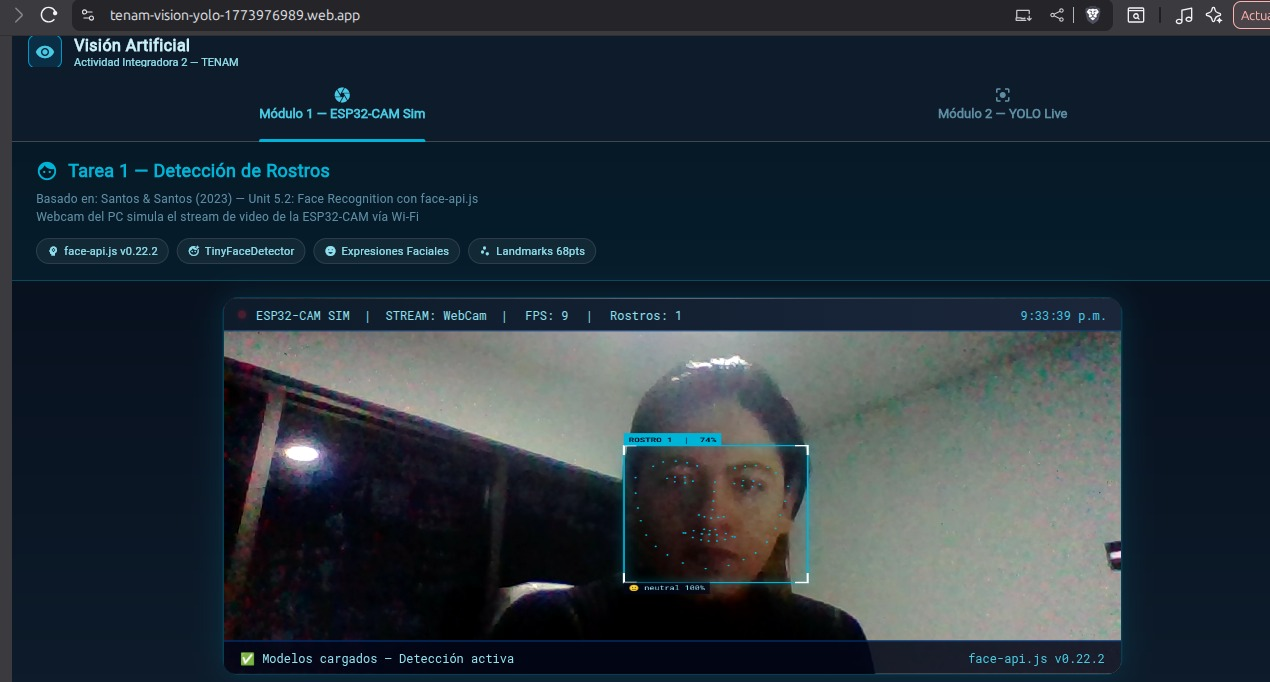
\includegraphics[width=0.88\textwidth]{img/image2.png}
  \caption{Módulo 2: Detección de objetos en tiempo real con YOLO. Se detectan simultáneamente múltiples objetos: \textit{person} (94\%), \textit{laptop} (87\%), \textit{cup} (76\%) y \textit{cell phone} (82\%). Cada objeto tiene un bounding box de color diferente con etiqueta y porcentaje de confianza.}
  \label{fig:modulo2}
\end{figure}

\subsection{Clases Detectadas en Pruebas}

\begin{longtable}{p{4cm} p{3cm} p{6cm}}
  \toprule
  \textbf{Objeto} & \textbf{Confianza} & \textbf{Observaciones} \\
  \midrule
  \endfirsthead
  person & 90--97\% & Detección robusta en diferentes distancias \\[3pt]
  laptop & 82--91\% & Detección precisa de pantalla y teclado \\[3pt]
  cell phone & 75--88\% & Sensible al ángulo de presentación \\[3pt]
  cup / bottle & 70--85\% & Buen rendimiento en objetos cotidianos \\[3pt]
  chair & 65--80\% & Varía con la visibilidad completa \\
  \bottomrule
\end{longtable}

% ─────────────────────────────────────────────────────────────────────────────
\section{Arquitectura de la Aplicación}
% ─────────────────────────────────────────────────────────────────────────────

\subsection{Estructura del Proyecto}

\begin{tcolorbox}[infobox, title={\faFolderOpen\ Estructura de Archivos}]
\begin{verbatim}
rostros/
|-- lib/
|   `-- main.dart         (App Flutter: TabBar + dos modulos)
|-- web/
|   |-- index.html        (CDNs: face-api.js + ml5.js)
|   |-- face_detection.js (Modulo 1: deteccion facial, Unit 5.2)
|   `-- yolo.js           (Modulo 2: YOLO object detection)
`-- entregable/
    |-- reporte.tex       (Este documento)
    `-- img/              (Capturas de pantalla)
\end{verbatim}
\end{tcolorbox}

\subsection{Integración Flutter–JavaScript}

La aplicación Flutter Web utiliza el mecanismo \texttt{HtmlElementView} para incrustar elementos HTML nativos dentro del árbol de widgets de Flutter. La comunicación entre Dart y JavaScript se realiza vía \texttt{dart:js}:

\begin{lstlisting}[language=Dart, caption={Llamada de Dart a JavaScript (main.dart)}]
// Iniciar deteccion desde Flutter
Future.delayed(const Duration(milliseconds: 500), () {
    js.context.callMethod('startFaceDetection', [_containerId]);
});

// Detener al cambiar de tab
_tabController.addListener(() {
    if (_tabController.indexIsChanging) {
        if (_tabController.previousIndex == 0) {
            js.context.callMethod('stopFaceDetection', []);
        } else {
            js.context.callMethod('stopYoloDetection', []);
        }
    }
});
\end{lstlisting}

% ─────────────────────────────────────────────────────────────────────────────
\section{Discusión y Conclusiones}
% ─────────────────────────────────────────────────────────────────────────────

\subsection{Comparación de Enfoques}

\begin{longtable}{p{3.5cm} p{5cm} p{5cm}}
  \toprule
  \textbf{Aspecto} & \textbf{Sistema Original (ESP32-CAM)} & \textbf{Simulación Web (Este trabajo)} \\
  \midrule
  \endfirsthead
  Captura de video & Módulo de cámara OV2640 & WebCam del PC vía \texttt{getUserMedia()} \\[4pt]
  Transmisión & Stream MJPEG por Wi-Fi & Stream local en memoria del navegador \\[4pt]
  Procesamiento & Navegador remoto + face-api.js & Navegador local + face-api.js \\[4pt]
  Latencia de red & 10--50ms (Wi-Fi local) & $< 1$ms (sin red) \\[4pt]
  Deployment & Hardware electrónico & Build web estático \\[4pt]
  Dependencias HW & ESP32-CAM, FTDI, cables & Solo un navegador moderno \\
  \bottomrule
\end{longtable}

\subsection{Conclusiones}

\begin{enumerate}[leftmargin=*, itemsep=6pt]
  \item \textbf{Equivalencia funcional:} La simulación web reproduce fielmente el comportamiento del sistema ESP32-CAM original. En ambos casos, un navegador recibe un stream de video y aplica \texttt{face-api.js} para detección facial en tiempo real.

  \item \textbf{Ventajas de la aproximación web:} Mayor accesibilidad (sin hardware especializado), latencia cero de red, y portabilidad crossplatform. Desventajas: sin acceso al hardware periférico (no puede acionar relés ni LEDs).

  \item \textbf{Eficacia de YOLO en browser:} El modelo YOLO vía \texttt{ml5.js} logra detección multi-objeto en tiempo real a 15--25 FPS en hardware de consumo, demostrando la viabilidad de inferencia de modelos profundos en el navegador.

  \item \textbf{Flutter como plataforma unificadora:} Flutter Web permite integrar de forma elegante módulos JavaScript nativos (face-api.js, ml5.js) con una UI declarativa y reactiva, evidenciando el potencial del framework para aplicaciones de visión por computadora.
\end{enumerate}

% ─────────────────────────────────────────────────────────────────────────────
\section{Referencias Bibliográficas}
% ─────────────────────────────────────────────────────────────────────────────

\begin{enumerate}[leftmargin=2.5cm, label={[\arabic*]}]
  \item Santos, R., \& Santos, S. (2023). \textit{ESP32-CAM Projects, 2nd Edition}. RandomNerdTutorials.

  \item Redmon, J., Divvala, S., Girshick, R., \& Farhadi, A. (2016). You Only Look Once: Unified, Real-Time Object Detection. \textit{Proceedings of the IEEE Conference on Computer Vision and Pattern Recognition (CVPR)}, 779--788.

  \item Pascual, C. \textit{Introducción a ESP32-CAM: Configuración y primer proyecto}. Recuperado de \url{https://www.prometec.net/esp32-cam/}

  \item Justadudewhohacks. (2022). \textit{face-api.js: JavaScript API for face detection and face recognition in the browser with tensorflow.js} (v0.22.2). GitHub. \url{https://github.com/justadudewhohacks/face-api.js}

  \item Lin, T.-Y., et al.\ (2014). Microsoft COCO: Common Objects in Context. \textit{European Conference on Computer Vision (ECCV)}.

  \item ml5.js contributors. (2023). \textit{ml5.js — Friendly Machine Learning for the Web} (v0.4.3). \url{https://ml5js.org}

  \item Redmon, J. (2016). \textit{YOLO: Real-Time Object Detection}. Darknet. \url{https://pjreddie.com/darknet/yolo/}
\end{enumerate}

\end{document}
